\section{Domain Analysis}

\subsection{Objective of the Laboratory Work}

The objective of this laboratory work is to implement an embedded PID control system for a physical process. The selected application is temperature regulation by forced ventilation: a DHT22 sensor measures the ambient temperature, the user selects the desired temperature setpoint, and a DC fan driven through an H-bridge receives a PWM command computed by a proportional-integral-derivative controller.

The work is prepared primarily for a real Arduino Mega 2560 setup. Wokwi is kept as a reproducible wiring and firmware reference for the supported logic-side components, but the L293D/L298-style motor driver, external 9 V supply, and fan branch must be validated on the physical circuit. This choice follows the provided hardware image, where the fan is powered separately from the Arduino logic rail and receives only control signals from the MCU.

\subsection{Problem Definition}

\begin{quote}
\small
``Să se proiecteze și să se implementeze o aplicație modulară pentru microcontroler (MCU) care realizează controlul PID asupra unui parametru fizic. Sistemul va achiziționa periodic valoarea parametrului de la un senzor adecvat, va compara cu valoarea de referință configurabilă și va calcula acțiunea de control utilizând algoritmul PID. Parametrii PID vor fi configurabili din cod sau din interfață, iar valorile parametrului măsurat, ale Set Point-ului, ale semnalului de control și starea actuatorului vor fi afișate pe LCD și/sau prin interfața serială.''
\end{quote}

The implemented system uses the DHT22 temperature as the measured process value and the fan speed as the manipulated output. Because the fan cools the environment, the controller is configured in reverse action: the error used by the PID algorithm increases when the measured temperature rises above the setpoint. The resulting control signal is limited to the range 0--100\%, then converted to a PWM duty cycle for the fan driver.

The setpoint is configurable through two mechanisms. The potentiometer on A0 provides the default continuous setpoint over the 18--35\textdegree C range. The 4x4 keypad can switch to manual mode, increment or decrement the manual setpoint, or confirm a numeric setpoint entry. The PID coefficients are configured in code and can also be changed at runtime through keypad-selected presets named SOFT, NORM, and FAST.

\subsection{Technical Requirements and Validation Criteria}

\begin{table}[H]
\centering
\begin{tabular}{|p{1.0cm}|p{7.2cm}|p{5.4cm}|}
\hline
\textbf{ID} & \textbf{Requirement} & \textbf{Validation Criterion} \\
\hline
R1 & Acquire temperature and humidity from the DHT22 without blocking unrelated application logic. & LCD and serial channels update after each acquisition cycle; invalid samples set `Valid:0`. \\
\hline
R2 & Provide a configurable temperature setpoint through potentiometer and keypad input. & A0 changes `SetPoint`; keypad manual entry overrides the potentiometer after confirmation. \\
\hline
R3 & Compute a bounded PID output from setpoint, measured value, and configured gains. & Serial Plotter shows `Output`, `Error`, `Kp`, `Ki`, and `Kd`; output remains between 0 and 100\%. \\
\hline
R4 & Apply the PID output to a PWM fan actuator through an H-bridge driver. & Fan duty follows `Duty`; the motor is stopped when the sensor is invalid or the PID output is near zero. \\
\hline
R5 & Separate acquisition, control, actuation, input, and display into FreeRTOS tasks. & Source tree contains dedicated task files and uses semaphores/mutexes for coordination. \\
\hline
R6 & Report process values for real-time analysis. & Arduino Serial Plotter receives named fields `SetPoint`, `Value`, `Output`, `Duty`, and `Error`. \\
\hline
\end{tabular}
\caption{Technical requirements and validation criteria}
\label{tab:requirements_validation}
\end{table}

\subsection{Used Technologies}

\subsubsection{PID Control}

The PID controller computes a continuous control signal from the current regulation error. The proportional term reacts to the current error, the integral term accumulates past error in order to reduce steady-state offset, and the derivative term reacts to the rate of change of the error. In discrete embedded software the controller is evaluated at a known sampling interval:
\[
u(k)=K_p e(k)+K_i \sum e(k)\Delta t+K_d\frac{e(k)-e(k-1)}{\Delta t}
\]
where \(u(k)\) is the command signal, \(e(k)\) is the current error, and \(K_p\), \(K_i\), and \(K_d\) are the configured gains.

For this cooling application the controller uses reverse action:
\[
e(k)=T_{measured}(k)-T_{setpoint}(k)
\]
so the fan command increases only when the measured temperature is higher than the desired value. The output is clamped to the physical range 0--100\% and the integral contribution is also clamped to reduce windup when the output saturates.

\begin{figure}[H]
\centering
\IfFileExists{resources/DomainAnalysis/UsedTechnologies/pid_control_loop.png}{%
    \includegraphics[width=0.72\textwidth]{resources/DomainAnalysis/UsedTechnologies/pid_control_loop.png}%
}{%
    \fbox{\parbox{0.70\textwidth}{\centering\color{gray}\small
        [Image pending --- save to resources/DomainAnalysis/UsedTechnologies/pid\_control\_loop.png]}}%
}
\caption{PID closed-loop control concept}
\label{fig:pid_control_loop}
\end{figure}

\subsubsection{PWM Motor Control}

Pulse-width modulation controls the average voltage applied to a DC motor by switching the driver rapidly between ON and OFF states. The Arduino `analogWrite` function produces an 8-bit PWM command from 0 to 255, which is mapped in the firmware from a duty cycle expressed as a percentage. The motor driver receives a PWM enable signal and two direction inputs. In this lab the fan is operated in one direction only, therefore IN1 is held HIGH, IN2 is held LOW, and the enable pin receives the PID-controlled duty cycle.

\subsubsection{I2C LCD Interface}

The LCD 1602 display uses an I2C backpack, so it requires only SDA, SCL, 5 V, and GND. The same I2C interface is used in the previous laboratories and is reused here to display current temperature, setpoint, fan duty, PID error, and selected gain preset.

\begin{figure}[H]
\centering
\IfFileExists{resources/DomainAnalysis/UsedTechnologies/i2c_protocol.png}{%
    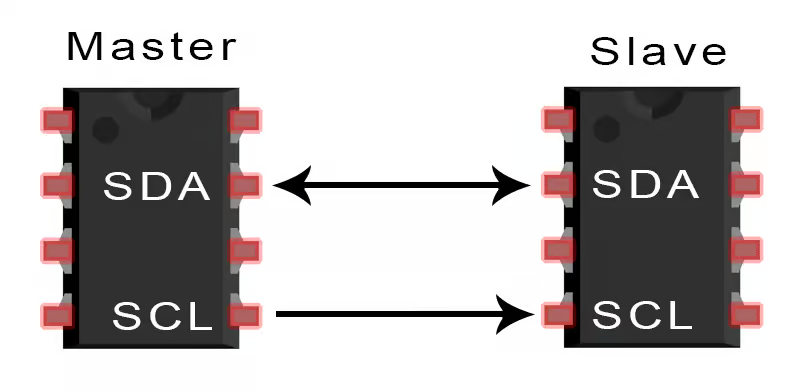
\includegraphics[width=0.72\textwidth]{resources/DomainAnalysis/UsedTechnologies/i2c_protocol.png}%
}{%
    \fbox{\parbox{0.70\textwidth}{\centering\color{gray}\small
        [Image pending --- save to resources/DomainAnalysis/UsedTechnologies/i2c\_protocol.png]}}%
}
\caption{I2C protocol used by the LCD module}
\label{fig:i2c_protocol}
\end{figure}

\subsubsection{FreeRTOS Task Scheduling}

FreeRTOS is used to separate periodic and event-driven responsibilities. The input task scans the keypad every 50 ms, the acquisition task samples the DHT22 and potentiometer every 2000 ms, the control task waits for a new sample, the actuation task waits for a fresh control command, and the display task updates the LCD and Serial Plotter every 500 ms. A mutex protects shared state and binary semaphores express the order acquisition \(\rightarrow\) control \(\rightarrow\) actuation.

\subsection{Hardware Components}

\subsubsection{Arduino Mega 2560}

The Arduino Mega 2560 provides enough GPIO for the keypad matrix, DHT22 data line, I2C LCD, potentiometer input, and H-bridge motor driver. Its PWM-capable D13 pin is used as the fan enable command, while D16 and D17 provide the fan direction signals.

\begin{figure}[H]
\centering
\IfFileExists{resources/DomainAnalysis/HardwareComponents/arduino_mega_2560.png}{%
    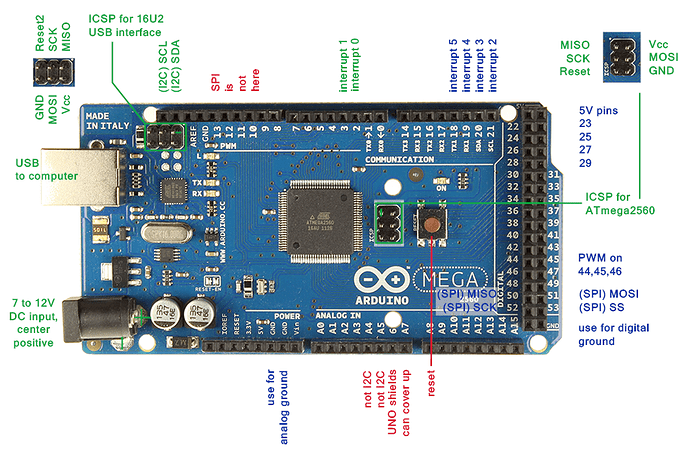
\includegraphics[width=0.62\textwidth]{resources/DomainAnalysis/HardwareComponents/arduino_mega_2560.png}%
}{%
    \fbox{\parbox{0.60\textwidth}{\centering\color{gray}\small
        [Photo pending --- save to resources/DomainAnalysis/HardwareComponents/arduino\_mega\_2560.png]}}%
}
\caption{Arduino Mega 2560 development board}
\label{fig:arduino_mega_2560}
\end{figure}

\subsubsection{DHT22 Temperature and Humidity Sensor}

The DHT22 sensor measures the process temperature and reports humidity as a diagnostic value. Its data line is connected to D2. A pull-up resistor is shown in the wiring reference because the data bus must return to logic HIGH between sensor transactions.

\begin{figure}[H]
\centering
\IfFileExists{resources/DomainAnalysis/HardwareComponents/dht22.png}{%
    \includegraphics[width=0.45\textwidth]{resources/DomainAnalysis/HardwareComponents/dht22.png}%
}{%
    \fbox{\parbox{0.43\textwidth}{\centering\color{gray}\small
        [Photo pending --- save to resources/DomainAnalysis/HardwareComponents/dht22.png]}}%
}
\caption{DHT22 temperature and humidity sensor}
\label{fig:dht22_sensor}
\end{figure}

\subsubsection{Potentiometer}

The potentiometer forms a voltage divider between 5 V and GND, and its wiper is connected to A0. The firmware maps the ADC value linearly to the allowed setpoint range, making it possible to test the controller without a computer-side command interface.

\begin{figure}[H]
\centering
\IfFileExists{resources/DomainAnalysis/HardwareComponents/potentiometer.png}{%
    \includegraphics[width=0.42\textwidth]{resources/DomainAnalysis/HardwareComponents/potentiometer.png}%
}{%
    \fbox{\parbox{0.40\textwidth}{\centering\color{gray}\small
        [Photo pending --- save to resources/DomainAnalysis/HardwareComponents/potentiometer.png]}}%
}
\caption{Potentiometer used for setpoint selection}
\label{fig:potentiometer}
\end{figure}

\subsubsection{4x4 Matrix Keypad}

The keypad provides local interaction. Key A toggles between potentiometer and manual setpoint mode, B and C decrease or increase the manual setpoint, D cycles the PID preset, digits enter a numeric setpoint, `\#` confirms the value, and `*` cancels the edit.

\begin{figure}[H]
\centering
\IfFileExists{resources/DomainAnalysis/HardwareComponents/keypad_matrix.png}{%
    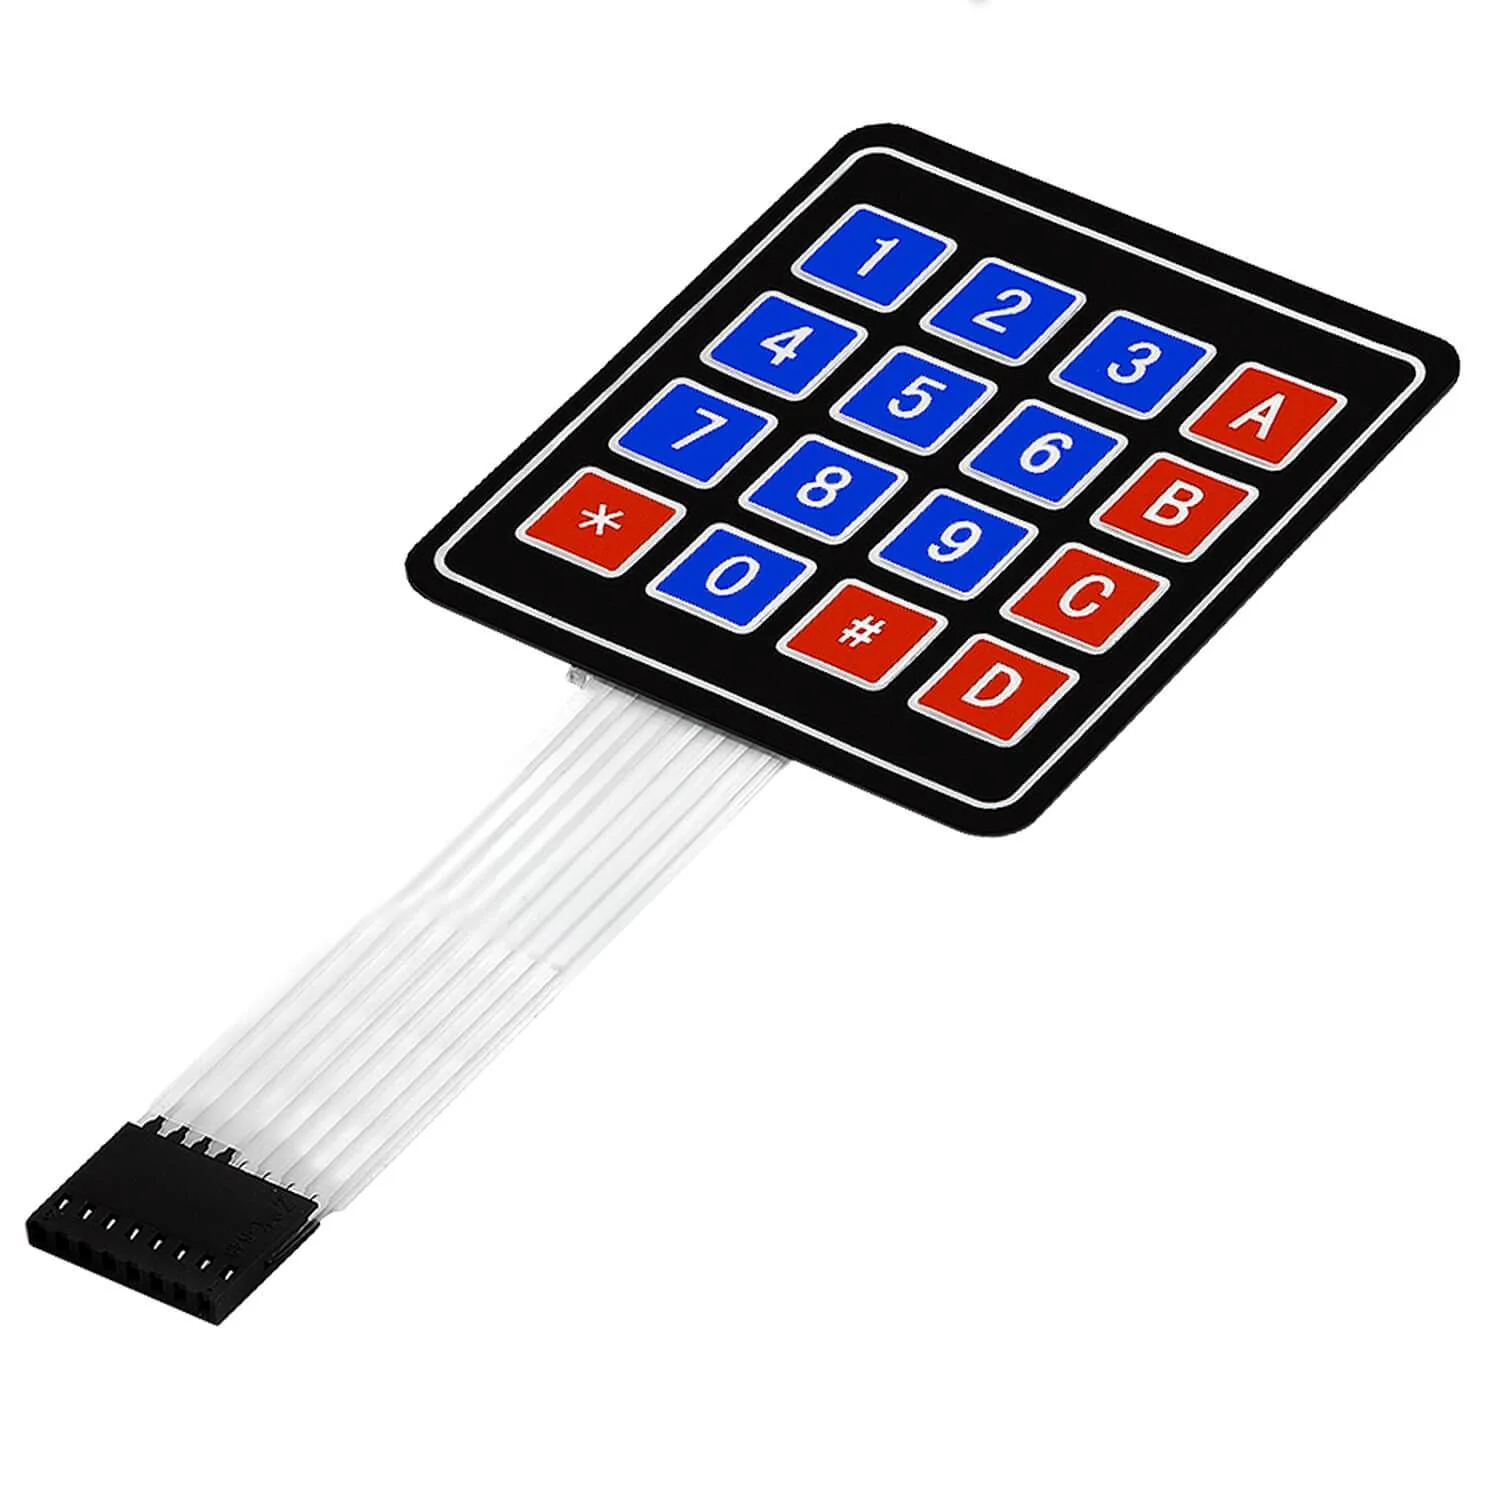
\includegraphics[width=0.45\textwidth]{resources/DomainAnalysis/HardwareComponents/keypad_matrix.png}%
}{%
    \fbox{\parbox{0.43\textwidth}{\centering\color{gray}\small
        [Photo pending --- save to resources/DomainAnalysis/HardwareComponents/keypad\_matrix.png]}}%
}
\caption{4x4 membrane matrix keypad}
\label{fig:keypad_matrix}
\end{figure}

\subsubsection{LCD 1602 I2C Display}

The LCD gives direct feedback during physical testing. It alternates between process values, controller error/output, and PID gains so the board can be operated without relying only on the Serial Plotter.

\begin{figure}[H]
\centering
\IfFileExists{resources/DomainAnalysis/HardwareComponents/lcd_1602_i2c.png}{%
    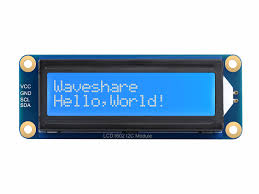
\includegraphics[width=0.48\textwidth]{resources/DomainAnalysis/HardwareComponents/lcd_1602_i2c.png}%
}{%
    \fbox{\parbox{0.46\textwidth}{\centering\color{gray}\small
        [Photo pending --- save to resources/DomainAnalysis/HardwareComponents/lcd\_1602\_i2c.png]}}%
}
\caption{LCD 1602 module with I2C backpack}
\label{fig:lcd_1602_i2c}
\end{figure}

\subsubsection{L293D/L298-Style H-Bridge Driver}

The motor driver isolates the Arduino logic pins from the higher-current fan load. The enable input receives PWM from D13, while D16 and D17 select the fan direction. The physical branch uses an external 9 V supply, so the Arduino GND and driver logic GND must share a reference.

\begin{figure}[H]
\centering
\IfFileExists{resources/DomainAnalysis/HardwareComponents/h_bridge_driver.png}{%
    \includegraphics[width=0.50\textwidth]{resources/DomainAnalysis/HardwareComponents/h_bridge_driver.png}%
}{%
    \fbox{\parbox{0.48\textwidth}{\centering\color{gray}\small
        [Photo pending --- save to resources/DomainAnalysis/HardwareComponents/h\_bridge\_driver.png]}}%
}
\caption{L293D/L298-style H-bridge motor driver}
\label{fig:h_bridge_driver}
\end{figure}

\subsubsection{DC Fan and External Supply}

The DC fan is the physical actuator. The 9 V source powers the motor side of the driver, while the Arduino only provides control logic and PWM. This separation is important because the fan current should not be drawn from the Arduino 5 V regulator.

\begin{figure}[H]
\centering
\IfFileExists{resources/DomainAnalysis/HardwareComponents/dc_fan.png}{%
    \includegraphics[width=0.45\textwidth]{resources/DomainAnalysis/HardwareComponents/dc_fan.png}%
}{%
    \fbox{\parbox{0.43\textwidth}{\centering\color{gray}\small
        [Photo pending --- save to resources/DomainAnalysis/HardwareComponents/dc\_fan.png]}}%
}
\caption{DC fan used as the PID-controlled actuator}
\label{fig:dc_fan}
\end{figure}

\subsection{Software Components}

PlatformIO is used to build the Arduino Mega firmware, manage external libraries, and select the active lab environment. Wokwi is used as a partial wiring reference for the logic-side circuit. Full actuator validation remains a physical test because the provided fan/driver branch is not completely represented in the simulator.

\begin{figure}[H]
\centering
\IfFileExists{resources/DomainAnalysis/SoftwareComponents/platformio.png}{%
    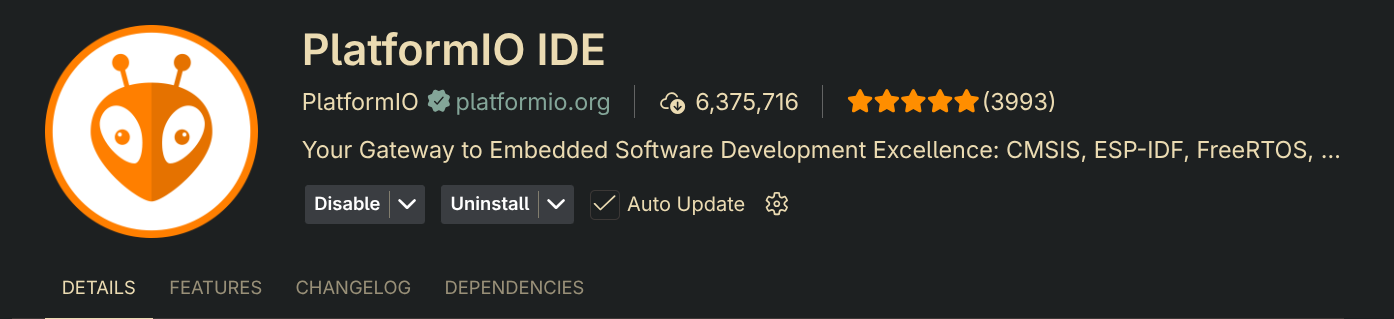
\includegraphics[width=0.75\textwidth]{resources/DomainAnalysis/SoftwareComponents/platformio.png}%
}{%
    \fbox{\parbox{0.73\textwidth}{\centering\color{gray}\small
        [Screenshot pending --- save to resources/DomainAnalysis/SoftwareComponents/platformio.png]}}%
}
\caption{PlatformIO development environment}
\label{fig:platformio}
\end{figure}

\begin{figure}[H]
\centering
\IfFileExists{resources/DomainAnalysis/SoftwareComponents/wokwi.png}{%
    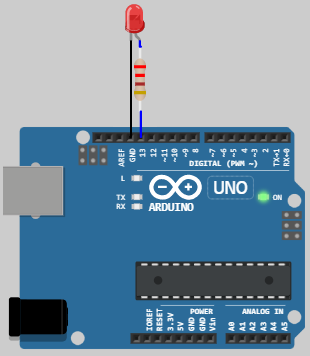
\includegraphics[width=0.75\textwidth]{resources/DomainAnalysis/SoftwareComponents/wokwi.png}%
}{%
    \fbox{\parbox{0.73\textwidth}{\centering\color{gray}\small
        [Screenshot pending --- save to resources/DomainAnalysis/SoftwareComponents/wokwi.png]}}%
}
\caption{Wokwi wiring reference environment}
\label{fig:wokwi}
\end{figure}

\subsection{Application Context}

PID temperature control is widely used in electronics cooling, incubators, environmental chambers, greenhouse ventilation, and process-control equipment. A fan-based controller is intentionally simple but demonstrates the same design pattern used in larger HVAC systems: measure the temperature, compare it with a setpoint, compute a continuous command, and apply the command through a power driver. The embedded implementation must also consider sensor update rate, actuator saturation, invalid measurements, and clear diagnostic reporting.
